The project intends to achieve the following outcomes:
\begin{itemize}
    \item Informative results on testing and evaluating the current payment system used at toll gates in comparison to the new proposed system
    \item A well developed and operational cross-platform mobile application to enable payment of toll fees as well as verification of the payments. This application will be available for both iOS and Android mobile platforms
    \item A functional embedded QR Code scanner that's able to capture QR code values and verify payments that have been made.

\end{itemize}


\section{Project Gaps and Future Works}
Currently, implementation of the project will be limited to the university scope and only accounts for users with smartphones with iOS and Android Operating Systems.

\begin{figure}
    \begin{center}
        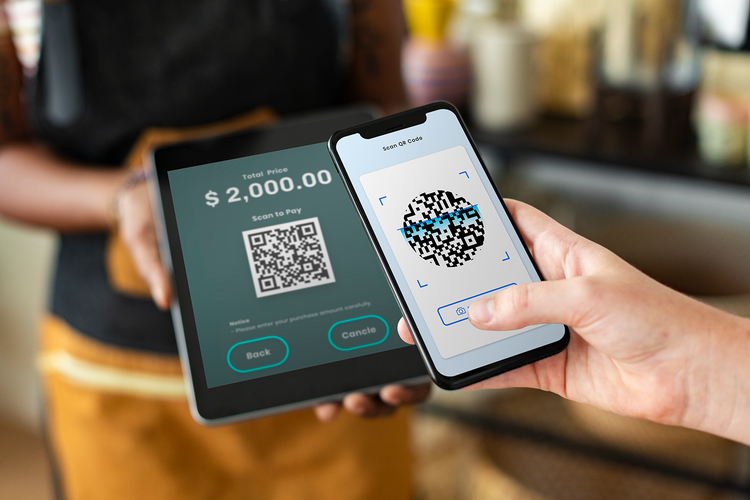
\includegraphics[scale = 0.6]{images/qr}
        \caption{The proposed system's payment will be limited to smartphones. In future, the project could be improved to support other phones}
    \end{center}
\end{figure}
This project can easily be scaled to various places such as malls and hospitals, and extended to account for non-smartphone users.


\clearpage
\bibliographystyle{IEEEtran}
\bibliography{references}
\begin{appendices}
    \textbf{Interview Questions: Motorist}
    \begin{itemize}
        \item What are some of the challenges you have faced using Makerere's toll gates?
        \item Describe the process of payment for toll fee at the ticket stations.
        \item How many times do you use the toll gate in a day?
        \item How much do you typically spend on toll gates?
        \item Do you often find queues at the toll gates?
        \item If you do, how often does this happen and at what times of the day?
    \end{itemize}

    \textbf{Interview Questions: Toll Operator}
    \begin{itemize}
        \item How many vehicles use this gate?
        \item What challenges do you normally face when using these gates?
        \item Do you believe cashless payments would ease your organisation's work?
    \end{itemize}
    \begin{figure}
        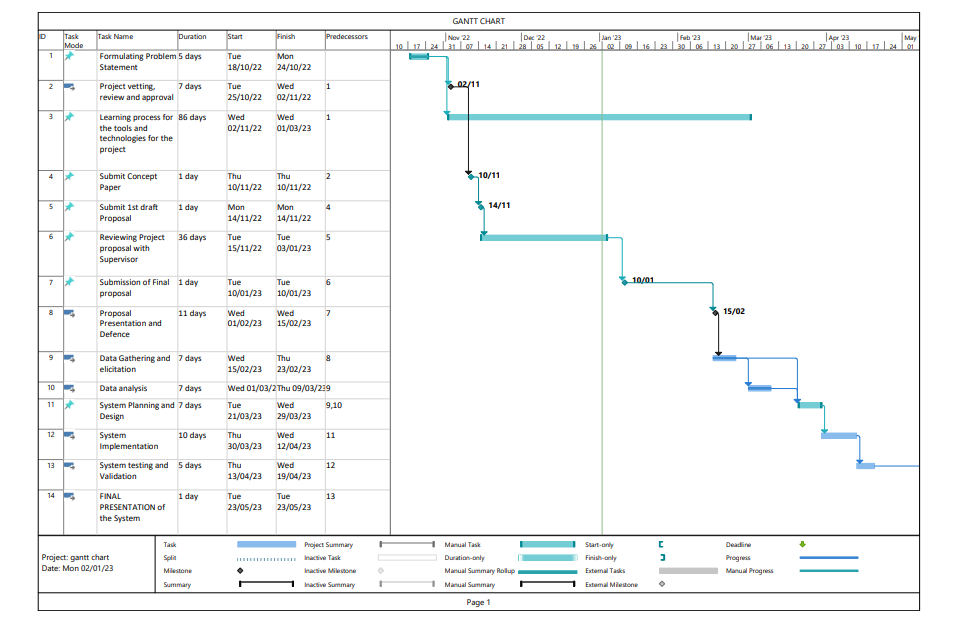
\includegraphics[scale = 0.6]{images/gantt}
        \caption{Gantt chart for execution of the project}
    \end{figure}
\end{appendices}